% !TeX spellcheck = en_US

\documentclass[a4paper,oneside,11pt]{memoir}

% Used to generate links, can be removed for final version
\usepackage{hyperref}
%used for \cref
\usepackage{cleveref}

%\usepackage{listings}

\newcommand{\shellcmd}[1]{\\\texttt{\footnotesize\# #1}}

% *** CITATION PACKAGE ***
\usepackage{cite}

% *** GRAPHICS RELATED PACKAGES ***
%
\usepackage[pdftex]{graphicx}
%   declare the path(s) where your graphic files are
\graphicspath{{../pdf/}{../jpeg/}}
%   and their extensions so you won't have to specify these with
%   every instance of \includegraphics
\DeclareGraphicsExtensions{.pdf,.jpeg,.png}

\usepackage{pgfplots}
\pgfplotsset{compat=1.8}
\usepgfplotslibrary{statistics}

\usepackage{filecontents}

\usepackage[caption=false,font=normalsize,labelfont=sf,textfont=sf]{subfig}



% *** PDF, URL AND HYPERLINK PACKAGES ***

\usepackage{url}

\hyphenation{op-tical net-works semi-conduc-tor}

\begin{document}

\title{Context-Aware Authentication \\ Using Bluetooth Low Energy}

\author{Stefan~Krause-Kj\ae r\\
        Thomas Thisgaard Steffensen\\
        and \\
        Theis Nickelsen% <-this % stops a space
}

\newcommand{\buildBoxPlot}[5]{
	\addplot+[
	blue,
    solid,
	boxplot prepared={
		median= #1,
		upper quartile=#2,
		lower quartile=#3,
		upper whisker=#4,
		lower whisker=#5
	},
	] coordinates {};
	
}

% make the title area
\maketitle
\clearpage

\begin{abstract}

This paper proposes a nearby-system authentication method using Receive Signal Strength Indicator (RSSI) of a Bluetooth Low Energy (BLE) device. 
The purpose of the method is to give the user a seamless authentication experience and save the user time when logging in. 
The characteristics of an iPhone 5's RSSI value at different distances and in different environments were analyzed in preliminary experiments. 
Because of the noisy results from the preliminary experiments we propose to use a combination of a median filter and a hysteresis threshold to achieve stable values as a means for authentication.
A proof of concept application was developed proving that it is possible to seamlessly authenticate a user based on RSSI if the application is calibrated to the surrounding environment.

\end{abstract}

\clearpage

\tableofcontents
\clearpage

\include{sections/01_Introduction}
\section{Background}

\subsection{Why use Bluetooth Low Energy (BLE) for proximity detection}


Experiments have been performed indicating that RSSI is a viable mean for proximity detection \cite{ref:Takashi}.  It is important to mention that we were tasked with implementing a Bluetooth based solution. Therefor we did not compare a Bluetooth based solution to other solutions, such as face detection.

It is important that the proximity detection is implemented without pairing any devices. This is to make the authentication as seamless as possbile, by saving the user from spending time pairing the devices manually.

Our options were Bluetooth Low Energy (BLE) or regular Bluetooth. BLE has been chosen over regular Bluetooth for this project for the following reasons:
\begin{itemize}
	\item BLE has Low power consumption. The Bluetooth device might need to be turned on for a long time, which is why it is crucial that the device can hod battery for a long time.
	\item BLE allows a small amount of communication without pairing devices, which allows the system to discover and receive addresses of the devices in the immediate vicinity. This enables the system to determine if a given device is registered to a user of the system without pairing with the device.
\end{itemize}

BLE is a fairly new standard and as such not all devices supports it yet. However this is outweighed by the what is gained from choosing BLE. 

Currently BLE is amongst other supported by a number of cell phones and wearables see \cref{table:devices}.

\begin{table}[!t]
\caption{Device descriptions}
\label{table:devices}
\centering
% Some packages, such as MDW tools, offer better commands for making tables
% than the plain LaTeX2e tabular which is used here.
\begin{tabular}{|p{2.3cm}|p{1.3cm}|p{3.8cm}|}
\hline
\textbf{Device} & \textbf{Hardware Support} & \textbf{Software Support}\\
\hline
iPhone 5, iPhone 5s (IOS7) & Yes & Yes\\
\hline
Nexus 5 \newline (Kitkat 4.4.2) & Yes & Partial \newline
Client profile (Android 4.3)
Server profile (planned)\\
\hline
Pebble Smartwatch (Pebble OS 2.0) & Yes & Server profile\\
\hline
\end{tabular}
\end{table}

\subsection{Security}

Authenticating a user when the user is close to the system introduces many security issues, which the system developer needs to address.
How close should the user be to the system in order to be authorized? What happens if there is multiple devices close to the system? Will this compromise the overall system security and is this acceptable?

The answers to these questions obviously depends on the system and an authentication model should be introduced.
One could imagine a partial login system where the user is only granted access to functionality, which does not need high level security, when the user is close and more functionality on top of what has already been given, when the user swipes a nfc card.
So in this case the user would only be granted access to lower level functionality, such as 'view-only', when being close the system.

Authorization happens without pairing of bluetooth devices.
This means authorization happens via the MAC address that the BLE device broadcasts and that the system has the MAC addresses of the user devices stored for user device recognition.



\subsection{Partial authentication model}
A login method has been developed to take different levels of trust into account.
As presented in \cref{fig_authentication_model} the authentication model has three levels of trust
\begin{itemize}
\item High (green)
\item Medium (yellow)
\item Low (red)
\end{itemize}

\begin{figure}[!t]
	\centering
	\includegraphics[width=2.5in]{img/authenticationModel}
	\caption{ Partial login and trust }
	\label{fig_authentication_model}
\end{figure}

High trust is obtained by authenticating with a combination of two of the three authentication methods.
As shown in \cref{table_data_access} a user is only able to view and edit sensitive data within the high trust area of the model.

Medium trust is obtained by authenticating with either a username/password or biometric authentication.
These two authentication methods is reasonable secure and are used universally for authentication.
A user that has obtained medium trust is able to view sensitive data but cannot edit or delete it.
With medium trust a user can view and edit non sensitive data.

Low trust is obtained by calm authentication with a Bluetooth enabled device.
A user with low trust can view personal non sensitive data like a name or a personal todo-list.
No edit or delete is allowed.

This model allows the user to be partially authenticated before any physical interaction.
The system gets the ability to recognize users and may for instance use that information to move a session started on one system to the current system so the user is able to seamlessly work on from the point the previous session ended.

\begin{table}[!t]
\caption{Data access}
\label{table_data_access}
\centering
% Some packages, such as MDW tools, offer better commands for making tables
% than the plain LaTeX2e tabular which is used here.
\begin{tabular}{|p{1.3cm}|p{2.0cm}|p{2.0cm}|p{2.0cm}|}
\hline
\textbf{Trust} & \textbf{Non sensitive personal data} & \textbf{Non sensitive data} & \textbf{Sensitive data}\\
\hline
\textbf{High} & Read/Write & Read/Write & Read/Write\\
\hline
\textbf{Medium} & Read/Write & Read/Write & Read\\
\hline
\textbf{Low} & Read & - & -\\
\hline
\end{tabular}
\end{table}


\section{Methods}

\subsection{RSSI authentication}

Existing methods

Proposed methods

\section{Experiments}

\subsection{Test setup}

On Raspberry pi and Ubuntu we used the official bluetooth stack BlueZ.
The devices needs to be configured to use Bluetooth LE, this is done by running the command ‘sudo hciconfig hci0 leadv’

\url{http://books.google.dk/books?id=-LMq0NhoEQgC&pg=PA358&lpg=PA358&dq=EnableGatt&source=bl&ots=AXu2znOEUw&sig=PjvPAADd4H3WInDAEFszw1MALr8&hl=da&sa=X&ei=uilyU6biJIz6yAOH94CQCg&ved=0CIsBEOgBMAk#v=onepage&q=EnableGatt&f=false}

\subsection{Scenarios}

The base scenario consists of a Raspberry Pi with custom software as the system.
This system is the static part of the test scenarios and from it distance to nearby devices are measured.
The devices in the test scenarios will be a collection of cell phones from different vendors and other wearables.
The devices will be both static and moving depending on the test scenario.


\subsubsection{Difference in RSSI from different devices}
The purpose of this experiment is to determine if and how much devices differs in RSSI value measured from the same distance. The distance from the user to the system is solely determined using the RSSI value and therefor it is interesting to see how the each device influences the distance.
	The following devices has been chosen for this experiment: An iPhone 5, a Rasberry Pi and a Nexus 5... 

\subsubsection{Single user moving towards system}
Plot RSSI pr. meter

Discover RSSI threshold for login

\subsubsection{Single user moving away from system}
Discover RSSI threshold for logout

\subsubsection{Multiple devices, user moving towards system, other}
Interferens?

\subsubsection{Multiple devices, two users moving towards the system}
Who will be authenticated first?

% !TeX spellcheck = en_GB
\section{Results}
\label{sec_results}

In the following we present the results from the two scenarios.

\subsection{Dynamic distance}

\begin{figure}		
	
	%\begin{tikzpicture}
%  \begin{axis}
%    [
%	xlabel=meter,
%	ylabel=dBm,
%	xtick={1, 2, 3, 4, 5, 6, 7, 8, 9, 10, 11, 12},
%    xticklabels={0, 2, 4, 6, 8, 10, 12, 14, 16, 18, 20},
%    boxplot/draw direction=y
%    ]
%    
%
%%"00,0"
%\buildBoxPlot{-46}{-45}{-61}{-71}{-44}
%%"00,5"
%%\buildBoxPlot{-57}{-55}{-59}{-61}{-54}
%%"01"
%%\buildBoxPlot{-68}{-67}{-69}{-75}{-65}
%%"02"
%\buildBoxPlot{-69}{-67}{-75}{-85}{-63}
%%"04"
%\buildBoxPlot{-70}{-69}{-71}{-74}{-67}
%%"06"
%\buildBoxPlot{-78}{-76}{-79}{-81}{-72}
%%"08"
%\buildBoxPlot{-78}{-77}{-83}{-90}{-76}
%%"10"
%\buildBoxPlot{-78}{-77}{-80}{-83}{-75}
%%"12"
%\buildBoxPlot{-80}{-77}{-82}{-86}{-75}
%%"14"
%\buildBoxPlot{-77}{-76}{-77}{-78}{-74}
%%"16"
%\buildBoxPlot{-81}{-80}{-82}{-84}{-78}
%%"18"
%\buildBoxPlot{-85}{-83}{-85}{-91}{-81}
%%"20"
%\buildBoxPlot{-84}{-84}{-85}{-88}{-81}
%
%\end{axis}
%	
%\end{tikzpicture}


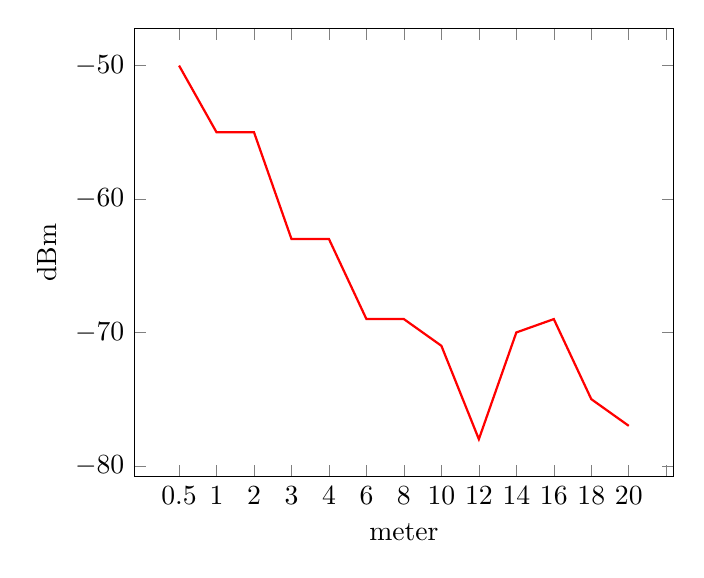
\begin{tikzpicture}
\begin{axis}
[
xlabel=meter,
ylabel=dBm,
xtick={1, 2, 3, 4, 5, 6, 7, 8, 9, 10, 11, 12, 13, 14},
xticklabels={0.5, 1, 2, 3, 4, 6, 8, 10, 12, 14, 16, 18, 20},
boxplot/draw direction=y
]


%"00.5"                                
\buildBoxPlot{-50}{-46}{-59}{-73}{-43} 
%%"00"                                  
%\buildBoxPlot{-26}{-26}{-27}{-30}{-25} 
%"01"                                  
\buildBoxPlot{-55}{-54}{-58}{-63}{-47} 
%"02"                                  
\buildBoxPlot{-55}{-48}{-58}{-79}{-44} 
%"03"                                  
\buildBoxPlot{-63}{-60}{-66}{-85}{-53} 
%"04"                                  
\buildBoxPlot{-63}{-60}{-68}{-89}{-51} 
%%"05"                                  
%\buildBoxPlot{-68}{-65}{-71}{-84}{-59} 
%"06"                                  
\buildBoxPlot{-69}{-67}{-71}{-90}{-61} 
%%"07"                                  
%\buildBoxPlot{-73}{-68}{-78}{-92}{-63} 
%"08"                                  
%\buildBoxPlot{-73}{-68}{-77}{-90}{-60} 
%%"09"                                  
\buildBoxPlot{-69}{-64}{-71}{-91}{-59} 
%"10"                                  
\buildBoxPlot{-71}{-67}{-75}{-92}{-62} 
%"12"                                  
\buildBoxPlot{-78}{-75}{-82}{-94}{-66} 
%"14"                                  
\buildBoxPlot{-70}{-68}{-73}{-81}{-60} 
%"16"                                  
\buildBoxPlot{-69}{-68}{-77}{-93}{-63} 
%"18"                                  
\buildBoxPlot{-75}{-71}{-78}{-93}{-65} 
%"20"                                  
\buildBoxPlot{-77}{-74}{-80}{-91}{-66} 


\addplot[thick, red] coordinates {
	(1  ,-50)
	(2  ,-55)
	(3  ,-55)
	(4  ,-63)	
	(5  ,-63)	
	(6  ,-69)	
	(7  ,-69)
	(8  ,-71)
	(9  ,-78)
	(10 ,-70)
	(11 ,-69)
	(12 ,-75)
	(13 ,-77)
	
	};
\end{axis}


\end{tikzpicture}

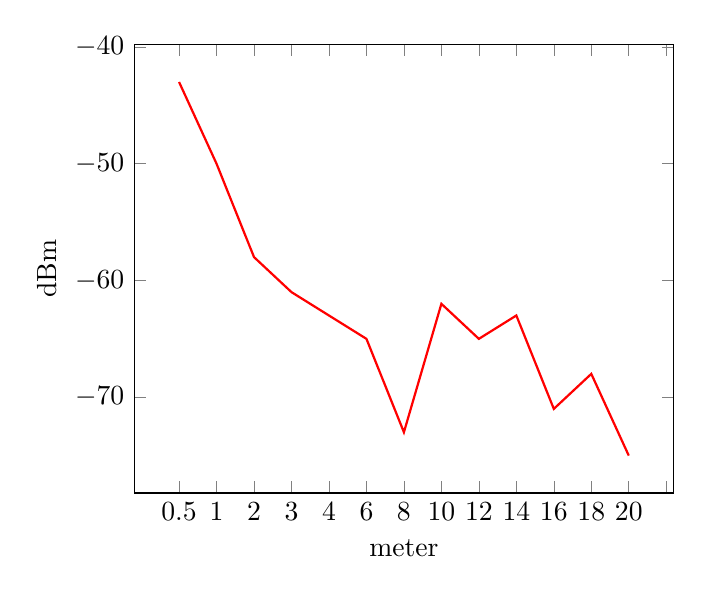
\begin{tikzpicture}
\begin{axis}
[
xlabel=meter,
ylabel=dBm,
xtick={1, 2, 3, 4, 5, 6, 7, 8, 9, 10, 11, 12, 13, 14},
xticklabels={0.5, 1, 2, 3, 4, 6, 8, 10, 12, 14, 16, 18, 20},
boxplot/draw direction=y
]


%%"00"
%\buildBoxPlot{-19}{-18}{-22}{-23}{-18}
%"00.5"
\buildBoxPlot{-43}{-42}{-45}{-49}{-41}
%"01"
\buildBoxPlot{-50}{-48}{-52}{-63}{-44}
%"02"
\buildBoxPlot{-58}{-53}{-62}{-81}{-46}
%"03"
\buildBoxPlot{-61}{-58}{-65}{-86}{-49}
%%"05"
%\buildBoxPlot{-64}{-62}{-66}{-80}{-55}
%"04"
\buildBoxPlot{-63}{-58}{-66}{-85}{-52}
%"06"
%\buildBoxPlot{-62}{-59}{-70}{-78}{-53}
%%"07"
\buildBoxPlot{-65}{-61}{-67}{-83}{-51}
%"08"
%\buildBoxPlot{-70}{-68}{-74}{-89}{-60}
%%"09"
\buildBoxPlot{-73}{-70}{-77}{-92}{-62}
%"12"
\buildBoxPlot{-62}{-61}{-64}{-75}{-57}
%"10"
\buildBoxPlot{-65}{-62}{-70}{-90}{-57}
%"16"
\buildBoxPlot{-63}{-62}{-65}{-71}{-56}
%"20"
\buildBoxPlot{-71}{-71}{-72}{-85}{-67}
%"14"
\buildBoxPlot{-68}{-64}{-71}{-81}{-57}
%"18"
\buildBoxPlot{-75}{-73}{-80}{-91}{-69}


\addplot[thick, red] coordinates {
	(1  ,-43)
	(2  ,-50)
	(3  ,-58)	
	(4  ,-61)	
	(5  ,-63)	
	(6  ,-65)
	(7  ,-73)
	(8  ,-62)
	(9 ,-65)
	(10 ,-63)
	(11 ,-71)
	(12 ,-68)
	(13 ,-75)
		
};

\end{axis}

\end{tikzpicture}

	
	\caption{ Dynamic distance measurements }
	\label{graf_DynamicMesurements}
	
\end{figure}

%\begin{figure}		
%	
%	\begin{tikzpicture}
  \begin{axis}
    [
	xlabel=meter,
	ylabel=dBm,
	xtick={1, 2, 3, 4, 5, 6, 7, 8, 9, 10, 11, 12},
    xticklabels={0, 2, 4, 6, 8, 10, 12, 14, 16, 18, 20},
    boxplot/draw direction=y
    ]
    

%"00,0"
\buildBoxPlot{-46}{ -45}{ -59}{ -63}{ -44}
%"00,5"
%\buildBoxPlot{-55}{ -55}{ -58}{ -60}{ -54}
%"01"
%\buildBoxPlot{-68}{ -67}{ -69}{ -72}{ -65}
%"02"
\buildBoxPlot{-70}{ -68}{ -74}{ -78}{ -65}
%"04"
\buildBoxPlot{-69}{ -69}{ -71}{ -72}{ -67}
%"06"
\buildBoxPlot{-78}{ -77}{ -78}{ -79}{ -73}
%"08"
\buildBoxPlot{-78}{ -77}{ -83}{ -83}{ -76}
%"10"
\buildBoxPlot{-78}{ -77}{ -79}{ -81}{ -75}
%"12"
\buildBoxPlot{-80}{ -78}{ -81}{ -84}{ -76}
%"14"
\buildBoxPlot{-77}{ -76}{ -77}{ -78}{ -75}
%"18"
\buildBoxPlot{-85}{ -83}{ -85}{ -89}{ -81}
%"16"
\buildBoxPlot{-81}{ -80}{ -81}{ -83}{ -78}
%"20"
\buildBoxPlot{-84}{ -83}{ -84}{ -87}{ -82}


\end{axis}
	
\end{tikzpicture}

%	
%	\caption{ Dynamic distance measurements Filtered }
%	\label{graf_DynamicMesurementsFiltered}
%	
%\end{figure}

The data from this scenario is presented in \cref{graf_DynamicMesurements}.
The figure shows RSSI value at 2 meter intervals between the base station and the mobile phone.
If we look at the median of the measurements there seems to be an exponential decreasing relation between distance and RSSI value.
We also see that measurements on the low side of the mean values has a wider distribution than on the high side of the mean measurements.

\subsection{Static distance}
\begin{figure}
	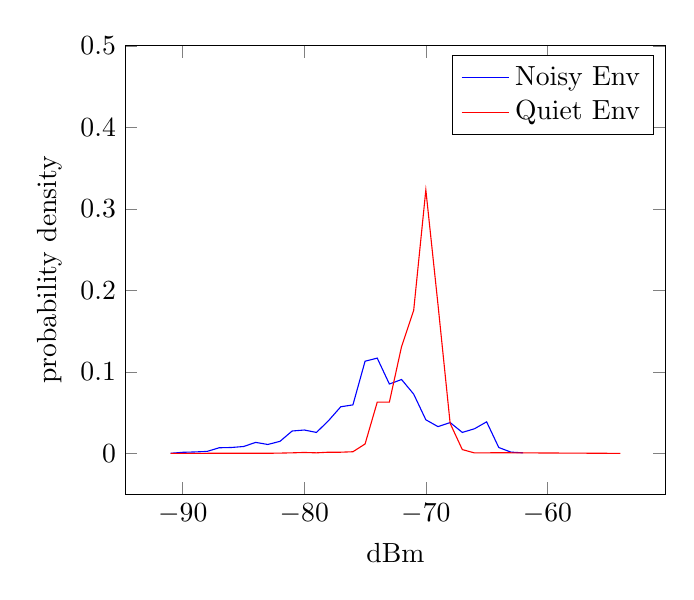
\begin{tikzpicture}
\begin{axis}[ymax=0.5,xlabel=dBm,ylabel=probability density]
\addplot[blue!20!blue] coordinates {
	(-91 ,0.0001093255)
	(-90 ,0.0013119055)
	(-89 ,0.0017492074)
	(-88 ,0.0024051602)
	(-87 ,0.0068875041)
	(-86 ,0.0072154805)
	(-85 ,0.0084180606)
	(-84 ,0.0134470318)
	(-83 ,0.0109325462)
	(-82 ,0.0147589374)
	(-81 ,0.0274406909)
	(-80 ,0.028643271)
	(-79 ,0.0256914835)
	(-78 ,0.04023177)
	(-77 ,0.0571772166)
	(-76 ,0.0594730513)
	(-75 ,0.1130425276)
	(-74 ,0.1168689188)
	(-73 ,0.0850552094)
	(-72 ,0.0906308079)
	(-71 ,0.0727014322)
	(-70 ,0.0412156991)
	(-69 ,0.0327976386)
	(-68 ,0.0378266098)
	(-67 ,0.0256914835)
	(-66 ,0.0301738275)
	(-65 ,0.0387012135)
	(-64 ,0.0072154805)
	(-63 ,0.0015305565)
	(-62 ,0.0006559528)

		};
\addplot[red!20!red] coordinates {
	(-91, 0)
	(-87, 0.0001107297)
	(-86, 0.0001107297)
	(-83, 0.0001107297)
	(-82, 0.0003321891)
	(-81, 0.0006643783)
	(-80, 0.0011072971)
	(-79, 0.0006643783)
	(-78, 0.0014394862)
	(-77, 0.0014394862)
	(-76, 0.0019931348)
	(-75, 0.0115158897)
	(-74, 0.0627837449)
	(-73, 0.0628944746)
	(-72, 0.1308825158)
	(-71, 0.1755065884)
	(-70, 0.3232200199)
	(-69, 0.1824825601)
	(-68, 0.0367622633)
	(-67, 0.0046506478)
	(-66, 0.0005536485)
	(-64, 0.000775108)
	(-54, 0)
	};
\legend{Noisy Env,Quiet Env}
\end{axis}
\end{tikzpicture}

	
	\caption{Static distance measurements}
	\label{graf_StaticMesurements}
\end{figure}

The data from this scenario is presented in \cref{graf_StaticMesurements}.
The figure shows how measurements are distributed over a period of 20 minutes when the distance between the base station and the mobile phone is static.
The experiment was performed in a quiet and a noisy environment.
As one would expect the RSSI values has a much higher spread in the noisy environment than in the quiet environment. 
 

\section{Discussion}
Seeing how the value of the RSSI measured from the device fluctuates in \cref{graf_DynamicMesurements} it is clear that RSSI is hard to use for distance measurements.
From a mean around 45 when measured right on top of the system the RSSI value drops drastically within the first few meters.
As the device moves further away from the system the RSSI value becomes lower but there is no apparent model to the decline.

The noise seams to fluctuate more towards the noise side of the mean. This suggests that if a lower value is measured it is more reliable then a high value, witch fits in well for authentication purposes.
Since most outliers are in the lower dBm end, there is a greater chance that you will be incorrectly logged out as a result of noise than incorrectly logged in.

Looking at \cref{graf_StaticMesurements} we clearly see that the RSSI value becomes less reliable the more noise there is in the environment.
The Noise level will affect how the hysteresis thresholds should be configured.
With too much noise in the environment the mean value of the graph will become indistinct from the rest.




\section{Conclusion}
Using RSSI value as viable means for proximity detection is possible but slightly inaccurate. Therefor we implemented a solution which uses a filter and a hysteresis threshhold combined, to remove noise from RSSI measureents and optimize accuracy, to make a more consistent proximity detection.

%
%A partial authentication model has been proposed taking the security aspect of calm authentication into consideration. The model has three levels of trust: Low, Medium and High allowing different read/write/edit rights according to the level of trust.

We have shown that context aware authentication using Bluetooth Low Energy is possible using RSSI measurements for proximity detection.

\section{Future work}
The following experiments would be interesting to consider for future work.


\subsection{Device RSSI value differences}

During this project we did not look into whether switching phone device would have an impact on the measured RSSI values.


\subsection{Multiple devices, user moving towards system, other}

The possibility of two users moving towards the same system is appearent. Therefor, to test how the RSSI value varies when multiple devices are near the system would be interesting.


\subsection{Time of Arrival (ToA)}
ToA is a method for measuring the distance between two objects, by measuring the time it takes a radio signal to travel between the objects. This is the same technique used in gps. ToA can provide reliable distance measurements but requires special hardware. This might serve as an interesting alternative to using the RSSI value of a Bluetooth device.



% if have a single appendix:
%\appendix[Proof of the Zonklar Equations]
% or
%\appendix  % for no appendix heading
% do not use \section anymore after \appendix, only \section*
% is possibly needed

% use appendices with more than one appendix
% then use \section to start each appendix
% you must declare a \section before using any
% \subsection or using \label (\appendices by itself
% starts a section numbered zero.)
%


%\appendices


%% use section* for acknowledgement
%\ifCLASSOPTIONcompsoc
%  % The Computer Society usually uses the plural form
%  \section*{Acknowledgments}
%\else
%  % regular IEEE prefers the singular form
%  \section*{Acknowledgment}
%\fi
%

%The authors would like to thank...


% Can use something like this to put references on a page
% by themselves when using endfloat and the captionsoff option.
%\ifCLASSOPTIONcaptionsoff
%  \newpage
%\fi


\input{sections/A_Referneces}

% trigger a \newpage just before the given reference
% number - used to balance the columns on the last page
% adjust value as needed - may need to be readjusted if
% the document is modified later
%\IEEEtriggeratref{8}
% The "triggered" command can be changed if desired:
%\IEEEtriggercmd{\enlargethispage{-5in}}

\include{sections/B_Biography}


% that's all folks
\end{document}

